%%
%% This is file `sample-authordraft.tex',
%% generated with the docstrip utility.
%%
%% The original source files were:
%%
%% samples.dtx  (with options: `authordraft')
%% 
%% IMPORTANT NOTICE:
%% 
%% For the copyright see the source file.
%% 
%% Any modified versions of this file must be renamed
%% with new filenames distinct from sample-authordraft.tex.
%% 
%% For distribution of the original source see the terms
%% for copying and modification in the file samples.dtx.
%% 
%% This generated file may be distributed as long as the
%% original source files, as listed above, are part of the
%% same distribution. (The sources need not necessarily be
%% in the same archive or directory.)
%%
%% The first command in your LaTeX source must be the \documentclass command.
\documentclass[sigconf,nonacm]{acmart}
\usepackage{src}
%% NOTE that a single column version may be required for 
%% submission and peer review. This can be done by changing
%% the \doucmentclass[...]{acmart} in this template to 
%% \documentclass[manuscript,screen,review]{acmart}
%% 
%% To ensure 100% compatibility, please check the white list of
%% approved LaTeX packages to be used with the Master Article Template at
%% https://www.acm.org/publications/taps/whitelist-of-latex-packages 
%% before creating your document. The white list page provides 
%% information on how to submit additional LaTeX packages for 
%% review and adoption.
%% Fonts used in the template cannot be substituted; margin 
%% adjustments are not allowed.
%%
%% \BibTeX command to typeset BibTeX logo in the docs
\AtBeginDocument{%
  \providecommand\BibTeX{{%
    \normalfont B\kern-0.5em{\scshape i\kern-0.25em b}\kern-0.8em\TeX}}}

%% Rights management information.  This information is sent to you
%% when you complete the rights form.  These commands have SAMPLE
%% values in them; it is your responsibility as an author to replace
%% the commands and values with those provided to you when you
%% complete the rights form.
\setcopyright{acmcopyright}
\copyrightyear{2023}
\acmYear{2023}
\acmDOI{10.1145/1122445.1122456}

%% These commands are for a PROCEEDINGS abstract or paper.
\acmConference[Woodstock '18]{Woodstock '18: ACM Symposium on Neural
  Gaze Detection}{June 03--05, 2018}{Woodstock, NY}
\acmBooktitle{Woodstock '18: ACM Symposium on Neural Gaze Detection,
  June 03--05, 2018, Woodstock, NY}
\acmPrice{15.00}
\acmISBN{978-1-4503-XXXX-X/18/06}


%%
%% Submission ID.
%% Use this when submitting an article to a sponsored event. You'll
%% receive a unique submission ID from the organizers
%% of the event, and this ID should be used as the parameter to this command.
%%\acmSubmissionID{123-A56-BU3}

%%
%% The majority of ACM publications use numbered citations and
%% references.  The command \citestyle{authoryear} switches to the
%% "author year" style.
%%
%% If you are preparing content for an event
%% sponsored by ACM SIGGRAPH, you must use the "author year" style of
%% citations and references.
%% Uncommenting
%% the next command will enable that style.
%%\citestyle{acmauthoryear}

%%
%% end of the preamble, start of the body of the document source.
\begin{document}

%%
%% The "title" command has an optional parameter,
%% allowing the author to define a "short title" to be used in page headers.
\title{The Evolution of Proof Assistant Math Repositories}

%%
%% The "author" command and its associated commands are used to define
%% the authors and their affiliations.
%% Of note is the shared affiliation of the first two authors, and the
%% "authornote" and "authornotemark" commands
%% used to denote shared contribution to the 

\author{Mahsa Bazzaz}
\affiliation{%
  \institution{Northeastern University}
  \city{Boston}
  \state{Massachusetts}
  \country{USA}
}

\author{Minsung Cho}
\affiliation{%
  \institution{Northeastern University}
  \city{Boston}
  \state{Massachusetts}
  \country{USA}
}

\author{Gwen Lincroft}
\affiliation{%
\institution{Northeastern University}
\city{Boston}
\state{Massachusetts}
\country{USA}}

%%
%% By default, the full list of authors will be used in the page
%% headers. Often, this list is too long, and will overlap
%% other information printed in the page headers. This command allows
%% the author to define a more concise list
%% of authors' names for this purpose.
\renewcommand{\shortauthors}{Bazzaz, Cho, and Lincroft}

%%
%% This command processes the author and affiliation and title
%% information and builds the first part of the formatted document.
\maketitle

\section{Introduction}

Proof assistants (also known as interactive theorem provers) are programming languages with the primary purpose of providing computational meaning to mathematical proof through code \cite{de2015lean}. The first proof assistants, developed over fifty years ago, were designed to help reason about the correctness of software and hardware through mathematical abstraction. However, as proof assistants became more expressive and user-friendly, they have gained traction in numerous fields, including formal methods, artificial intelligence, and computer science education \cite{green1981application,hunt1994fm8501,knobelsdorf2017theorem}.

However, over the past 20 years, proof assistants garnered attention from communities beyond computer science. In particular, the mathematics community took interests in proof assistants with their potential to bridge software development and mathematical proof. This potential has been realized through multiple open-source, well-documented libraries of formalized proofs as programs. Although there have been many such libraries over time, the predominant ones today are written in three languages: Lean, Coq, and Isabelle/HOL.

\textbf{Lean} has been the focal point of math library development in the past five years, gaining the attention of prominent mathematicians by demonstrating its ability to prove research-level mathematics \cite{buzzard_2020}. Its math library, known as \mathlib, has been open-sourced on GitHub under an Apache license. It has extremely rigid conventions for contributing, including guidelines on style, naming, commit messages, and pull request labeling. 

\textbf{Coq} is one of the most widely-used proof assistants in computer science today. However, its math library is not centralized like \mathlib. Instead, it offers a \textit{loosely federated} list of open-source GitHub repositories. Many of these repositories are under the same GitHub organizations, for example \texttt{math-comp} or \texttt{coq-community}, but not all of them are and their interdependence is not obvious.

\textbf{Isabelle/HOL} is another major proof assistant that offers an extremely strong general automation, which the other proof assistants lack. Although its math library is open source, it is not hosted natively on GitHub and external contribution is not done through GitHub's standard means. In particular, contribution is vetted behind closed doors by academics and is not done through a standard pull request-merge system. Furthermore, there is no centralized repository \'a la \mathlib and most are hosted on the website \textit{Archive of Formal Proofs}, where the proofs lack version control but give a detailed account of authors, dependencies, and proof techniques.

It is clear that each of these proof assistants and their math libraries have different software development practices. However, they all attempt to demonstrate the power of proof assistants by formalizing known mathematics through code. This project aims to compare and contrast the evolution of these three main repositories through a software engineering lens. In particular, for this project we have two main research questions:

\begin{enumerate}
    \item\label{r1} What mathematical theorems did different formalized mathematics libraries prove? How has this developed over time? How have the proofs changed?
    \item\label{r2} How has the popularity of contributing to theorem provers over time changed? Are there any factors we need to take into account to evaluate proof assistant software different than traditional software?
\end{enumerate}

\section{Project Results}

\subsection{Methodology}

To investigate research problem \ref{r1}, we used Freek Wiedijk's \textit{list of 100 theorems}\cite{wiedijk}, an online list of ``top 100'' mathematical theorems that proof assistants to attempt to formalize, which we will refer to as the \textit{100 Theorems list}.

We first gathered exactly what proportion of the 100 theorems have been formalized fully in the respective proof assistants. Then, we used \texttt{SimpleGit} to collect data of relevant commits to the file containing each theorem. For Lean, we collected data only from the \textit{mathlib} repository, where all the proofs were held. For Coq, we looked at 30 different repositories where the proofs were held. For Isabelle, we either looked at the \textit{mirror-afp-2022} repository or had to take data directly from the \textit{Archive of Formal Proofs} website.

Using the data, we selected the following information:
\begin{itemize}
 \item when each theorem was proven,
 \item which theorems required the most commits
 \item and what type of commits--code refactoring, dependency updating, or simply writing new supporting definitions and lemmas--were typically made.
\end{itemize}

To investigate the research problem \ref{r2}, we used \texttt{Octokit} to take data on pull requests and issues. However, this was only doable on Lean and Coq, as Isabelle does not have any pull requests or issues. We again used \texttt{SimpleGit} to collect data on commits. Using the data, we selected the following information:

\begin{itemize}
 \item the proportion of pull requests merged to the main or master branch, closed, and still open,
 \item the proportion of issues opened or closed,
 \item the number of unique contributors,
 \item the rate of growth of the repositories, measured as
 \begin{equation}\label{eq1}
   \#\text{ of commits}+\#\text{ of opened PRs}+\#\text{ of opened issues},
 \end{equation}
 \item the general type of pull request and issues seen in math repositories, such as suggestions, bugfixes, or new additions.
\end{itemize}

With this, we present our results.

\subsection{Results for research problem \ref{r1}}

We first observed that although Lean is the focal point of math library development in the past five years, Isabelle actually has the most theorems proved on the 100 Theorems list, with 87. Coq follows with 79, and Lean is actually the least populated with 76. Thus, in objective number of theorems proved, Lean is actually not the dominant proof assistant for formalized math. 

\begin{figure}[H]
  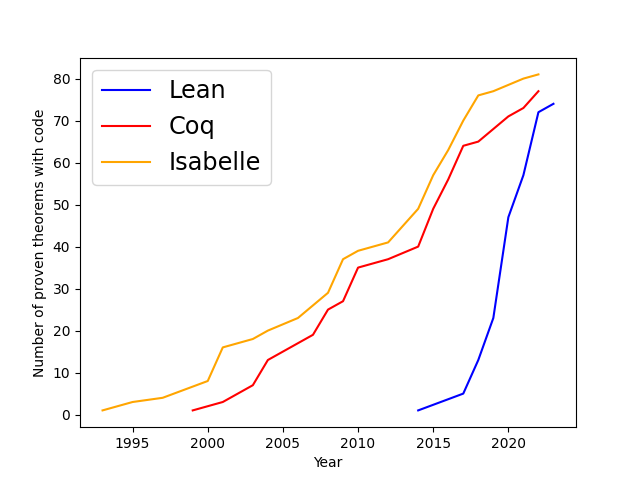
\includegraphics[scale=0.5]{thm_dev.png}
  \caption{Number of theorems on the 100 Theorems list proven via Lean/Coq/Isabelle over time.}
  \label{thms over time}
\end{figure}

However, Figure \ref{thms over time} demonstrates that Lean is catching up fast. Isabelle and Coq's main advantage is the longer history of development, which lends itself easily to more code. Furthermore, we see that Lean's \mathlib is growing significantly faster in the past five years than both Coq and Isabelle's libraries, with contributions even as recent as this year, which both Coq and Isabelle lack.

\begin{figure}[H]
  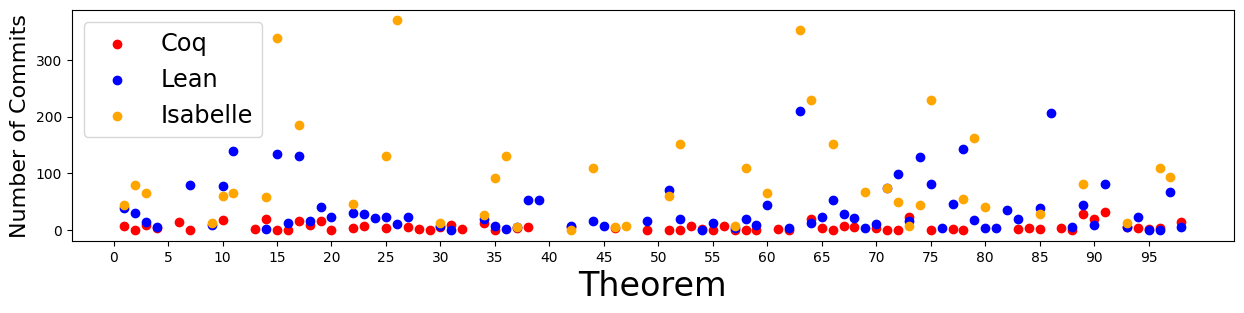
\includegraphics[scale=0.25]{test.png}
  \caption{Number of commits per proven theorem on the \textit{100 Theorems} list.}
  \label{number of commits}
\end{figure}

Figure \ref{number of commits} demonstrates that, although Coq has more theorems proven than Lean, per theorem it only has few commits. On the other hand, Isabelle seems to have many theorems with hundreds of commits to the source file. In general, we see little correlation between the different proof assistants and the number of commits to prove each theorem on the 100 Theorems list. 

We see in Figure \ref{historical commits} that there is also little correlation between the different proof assistants and the order in which the theorems were proven. However, we see a common pattern in all three proof assistants: there are times when several theorems are proven in a very short span of time. We believe this is due to similarities in the definitions and proof techniques used in the theorems rather than pure coincidence. Additionally, both Lean and Coq have instances of the same proof being proven in multiple implementations. We believe that this is due to the nature of the languages as a tool where the demonstration and exploration of a new capability or strategy is valued.

In general, the commit contents were mostly proofs of the theorem and related mathematics. We observed that often the theorems themselves are only consequences of an underlying theory, and not a standalone goal. This can be likened to mathematics, where usually theorems are consequences of studying an underlying theory and not a goal to build towards. We believe that this is also the reason why there is little correlation in the order in which theorems were proven and why theorems are proven multiple times. Besides proofs, other commit contents included dependency updates, refactoring of code, and comments to explain the proofs in English. We leave it to future work for a more sophisticated analysis of commit contents via code differences.

\begin{figure}[H]
  \begin{subfigure}{\columnwidth}
    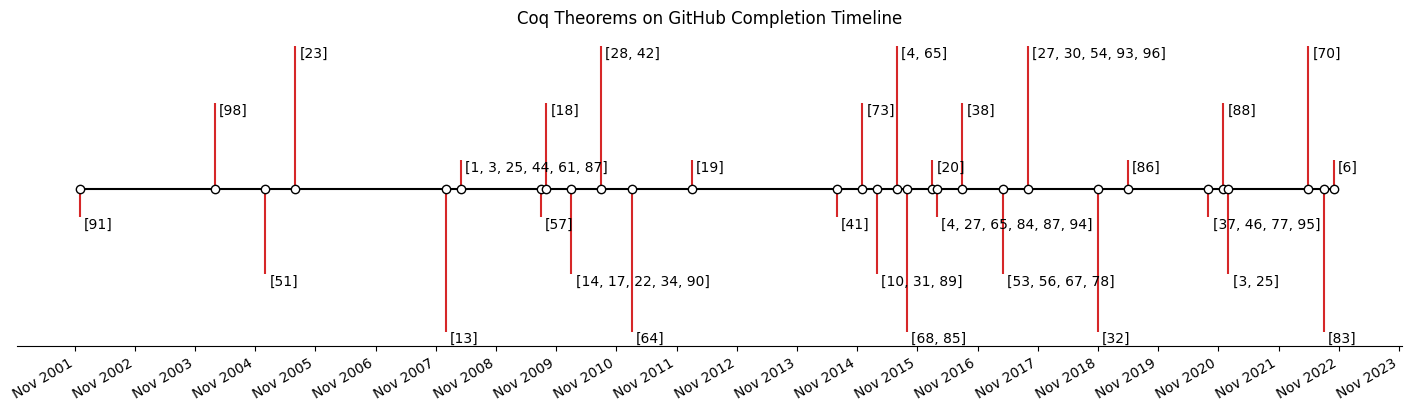
\includegraphics[width=\linewidth]{coq_theorems_timeline.png}
    \caption{Coq theorem timeline.}
  \end{subfigure}
  \begin{subfigure}{\columnwidth}
    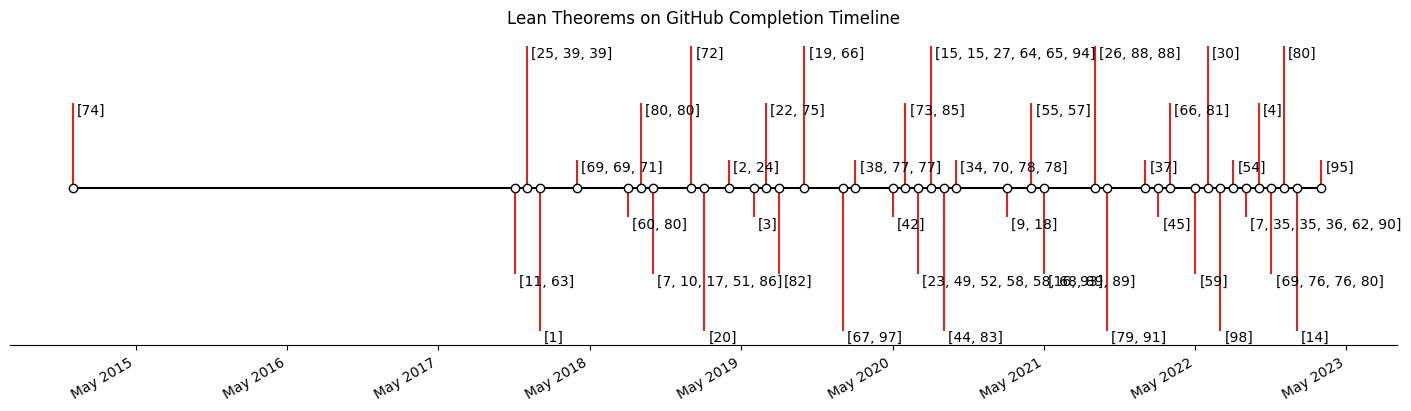
\includegraphics[width=\linewidth]{lean_theorems_timeline.png}
    \caption{Lean theorem timeline.}
  \end{subfigure}
  \begin{subfigure}{\columnwidth}
    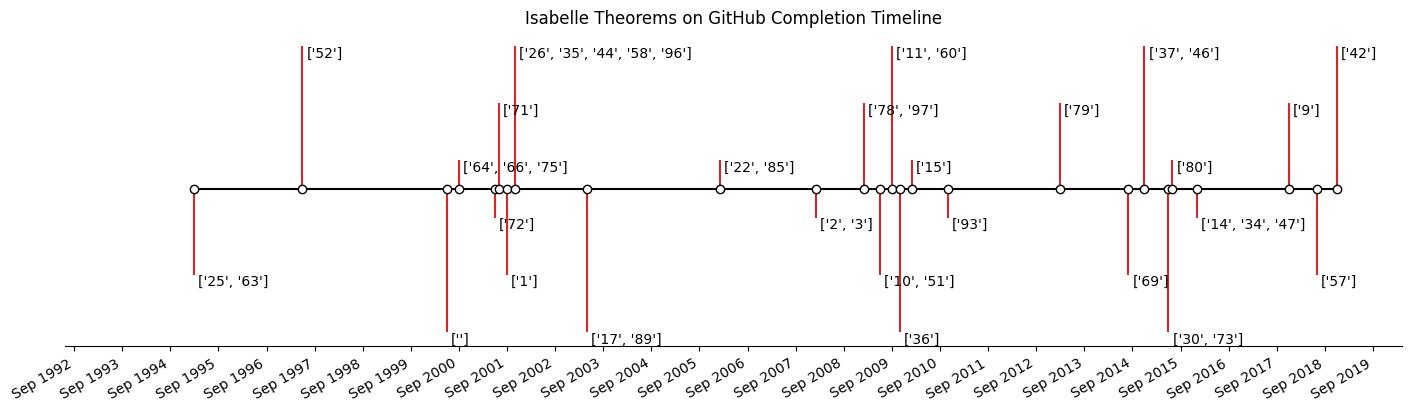
\includegraphics[width=\linewidth]{isabelle_theorems_timeline.png}
    \caption{Isabelle theorem timeline.}
  \end{subfigure}
  \caption{Theorems proved by Coq/Lean/Isabelle in chronological order. One point represents one month.}
  \label{historical commits}
\end{figure}

\subsection{Results for research problem \ref{r2}}

We observed in Figure \ref{thms over time} that Lean, in the context of math formalization, has exploded in growth over the past five years. We attempt to characterize this growth using different metrics derivable from looking at the history of Git activity for the proof assistants and their math libraries.

\begin{figure}[H]
  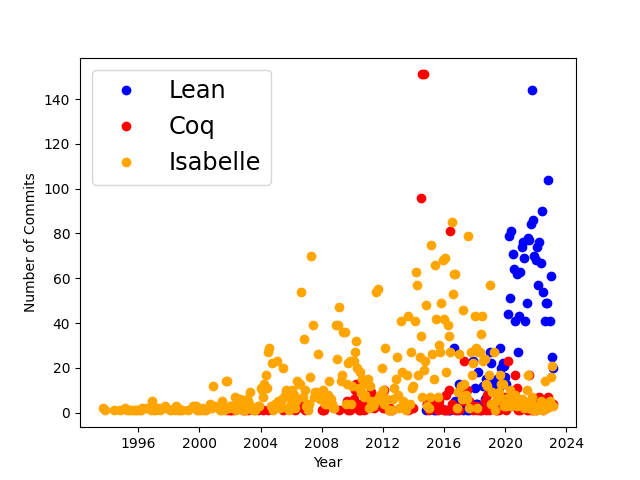
\includegraphics[scale=0.5]{compare_commits.png}
  \caption{Number of commits per year for Lean, Coq, and Isabelle.}
  \label{commits per year}
\end{figure}

We see in Figure \ref{commits per year} that in the past five years Lean has significantly more commits to its main repositories than both Coq and Isabelle. Before that, Isabelle had a commanding lead, although its activity seems to have diminished with the emergence of Lean. The slight increase in Isabelle activity in 2012-2016 corresponds to a large growth in proven theorems in Figure \ref{thms over time} over the same time frame.

Figure \ref{commits per year} also shows two outlier points for Coq: there are two points, occuring at August and September 2014, where the number of commits surpasses 300. Most of these commits were from one user and their solo project to prove Puiseux's Theorem, one of the theorems on the 100 Theorems list. Interestingly, none of the commit messages for these commits seem to have relevant information--the messages are simply "\texttt{--}".

\begin{figure}[H]
  \begin{subfigure}{\columnwidth}
    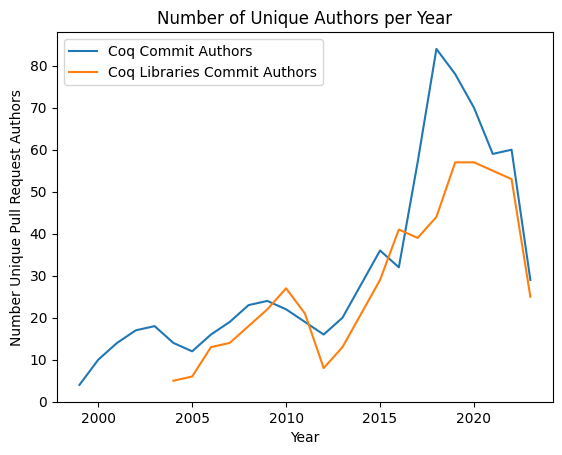
\includegraphics[scale=0.5]{coq_commit_authors.png}
    \caption{Number of unique Coq commit authors.}
  \end{subfigure}
  \begin{subfigure}{\columnwidth}
    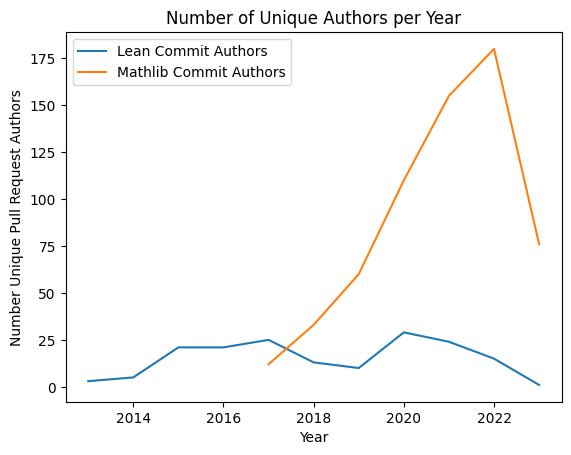
\includegraphics[scale=0.5]{lean_commits_authors.png}
    \caption{Number of unique Lean commit authors.}
  \end{subfigure}
  \begin{subfigure}{\columnwidth}
    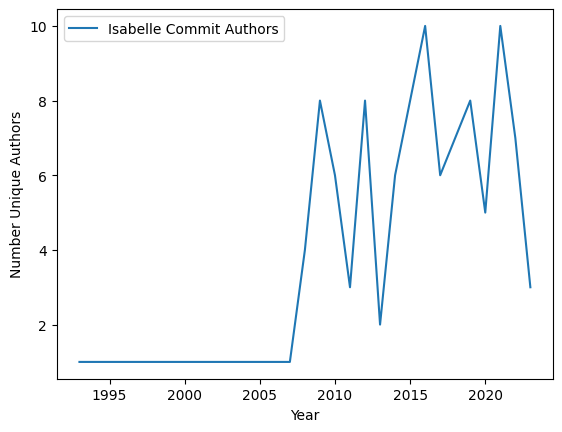
\includegraphics[scale=0.5]{isabelle_commit_authors.png}
    \caption{Number of unique Isabelle commit authors.}
  \end{subfigure}
  \caption{Number of unique authors contributing commits to languages and math libraries over time.}
  \label{Commit authors}
\end{figure}

Figure \ref{Commit authors} shows how changes to the main language libraries for Lean and Isabelle has been done by a small number of individuals, but many more people have contributed to the Coq language. Interestingly, in recent years, more people have contributed to the Coq language than to the sum of the federated Coq libraries. This indicates that while the implementation of Coq theorem provers is spread out, the Coq community is more centralized than it appears.

In contrast to Coq, the majority of recent contributors to Lean do not contribute to the Lean language and instead contribute to Lean libraries, such as Mathlib, as demonstrated in Figure \ref{Commit authors}. The Lean community is known for having strict contribution standards, but this does not appear to have affected the rapid increase in unique contributors to Mathlib.

The Isabelle repository contains not only the Isabelle language, but also each of the Isabelle proofs and the Isabelle math library. Figure \ref{Commit authors} shows that there are less committers for Isabelle than for all of Coq or Lean. For each commit made to Isabelle, what proportion of the changes originate from an individual who is not the committer? How many individuals work on a single commit? How might an Isabelle newcomer become a committer? These questions should be explored in future work.

\begin{figure}[H]
  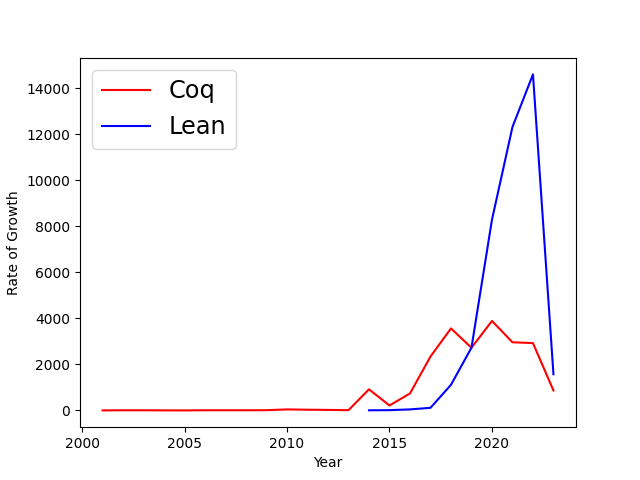
\includegraphics[scale=0.5]{rate.png}
  \caption{Rate of growth for Coq and Lean via Equation \ref{eq1}}
  \label{rate of growth}
\end{figure}

Figure \ref{rate of growth}, which shows code growth by Equation \ref{eq1} per year, reaffirms similar conclusions to Figure \ref{commits per year}. However, we noticed that Isabelle does not have a standard system for pull requests and issues. Instead, any changes in its library must be done through a form submitted to TU Munich, where Isabelle development is centered at. As such, the following analysis of pull requests and issues will be on Lean and Coq exclusively. 

\begin{figure}[H]
  \begin{subfigure}{0.45\columnwidth}
    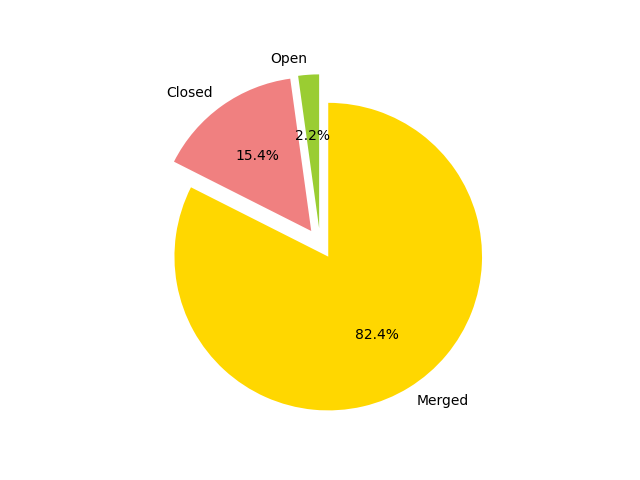
\includegraphics[width=\linewidth]{coq_prs_sate.png}
    \caption{Coq pull requests.}
    \label{coq prs}
  \end{subfigure}
  \hfill %%
  \begin{subfigure}{0.45\columnwidth}
    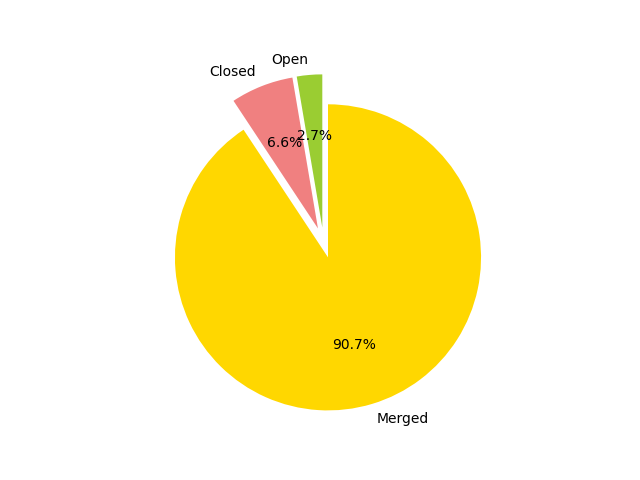
\includegraphics[width=\linewidth]{Lean_pull_requests_state.png}
    \caption{Lean pull requests.}
    \label{lean prs}
  \end{subfigure}
  \begin{subfigure}{0.45\columnwidth}
    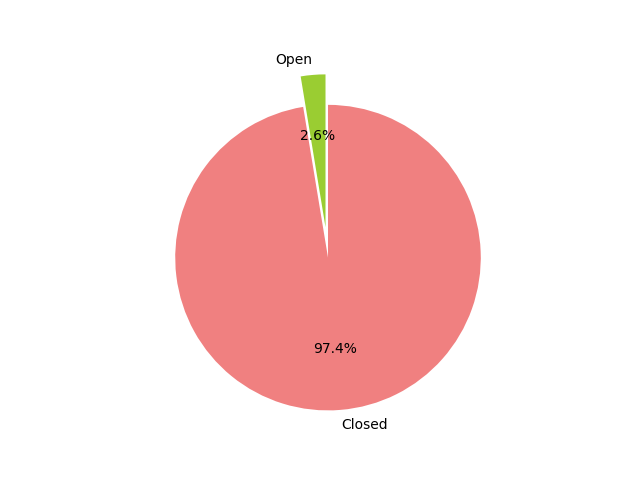
\includegraphics[width=\linewidth]{coq_isuses_state.png}
    \caption{Coq issues.}
    \label{coq issues}
  \end{subfigure}
  \hfill %%
  \begin{subfigure}{0.45\columnwidth}
    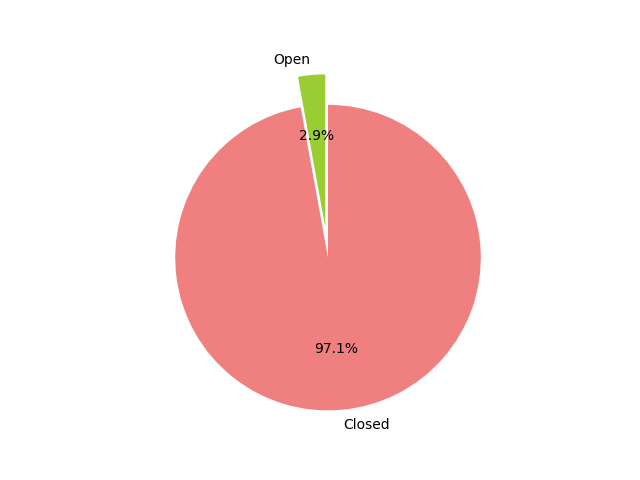
\includegraphics[width=\linewidth]{lean_isuses_state.png}
    \caption{Lean issues}
    \label{lean prs}
  \end{subfigure}
  \caption{The state of pull requests and issues for Coq and Lean. Red=closed, Green=open, Yellow=merged.}
  \label{circles}
\end{figure}

Figure \ref{circles} demonstrates that how Coq and Lean handle issues is relatively similar by proportion. It is interesting to note that although Lean arguably has more stringent style and pull request guidelines than Coq, its proportion of merged pull requests is slightly more than Coq. Indeed, Figure \ref{bars} reinforces the conclusion that although Coq and Lean are different in many ways, they follow similar open source guidelines.


\begin{figure}[H]
\begin{subfigure}{0.8\columnwidth}
  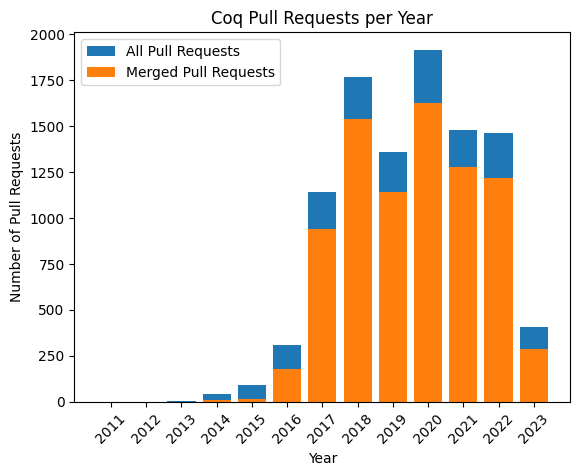
\includegraphics[width=\linewidth]{coq_mergedvsall.png}
  \caption{Coq.}
  \label{fig:1}
\end{subfigure}
\hfill %%
\begin{subfigure}{0.8\columnwidth}
  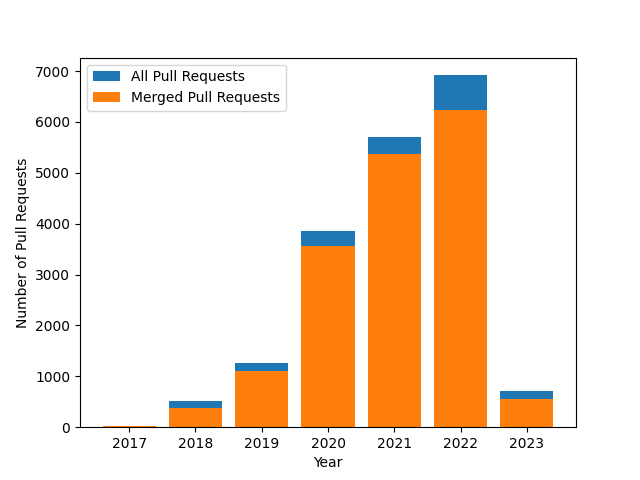
\includegraphics[width=\linewidth]{lean_mergedvsall.png}
  \caption{Lean.}
  \label{fig:2}
\end{subfigure}
\caption{All vs. merged pull requests for Coq and Lean.}
\label{bars}
\end{figure}

\begin{figure}[H]
\begin{subfigure}{0.8\columnwidth}
  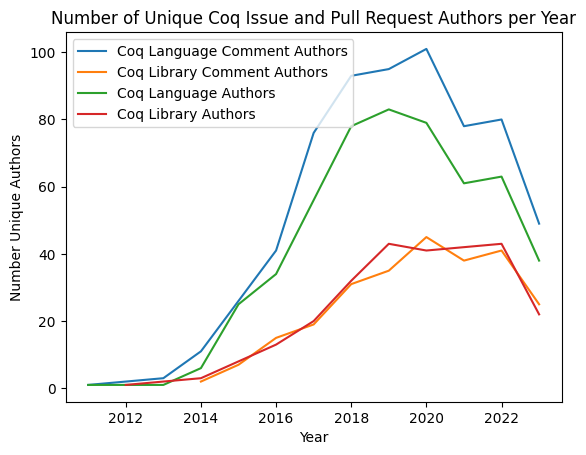
\includegraphics[width=\linewidth]{coq_ispr_authors.png}
  \caption{Coq.}
  \label{fig:1}
\end{subfigure}
\hfill %%
\begin{subfigure}{0.8\columnwidth}
  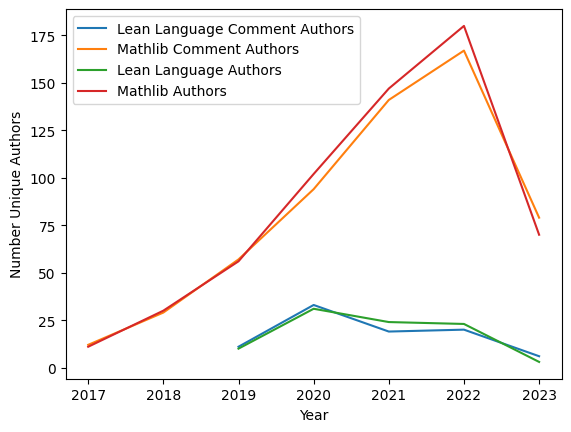
\includegraphics[width=\linewidth]{lean_ispr_authors.png}
  \caption{Lean.}
  \label{fig:2}
\end{subfigure}
\caption{Unique contributors to issues, pull requests, and related discussions in Coq and Lean}
\label{authors}
\end{figure}

Figure \ref{authors} shows the decline in overall community involvement in Coq post-2020 and the rapid growth of the Lean community. The sharp decline in unique authors in 2023 is a result of the year not yet being complete for both languages. Similarly to Figure \ref{Commit authors}, more unique community members contribute to the language in Coq than the proof libraries and more unique community members contribute to Mathlib in Lean than the Lean language.

\section{Project Challenges}

\subsection{Limits in project scope}

The original goal of this project was to investigate proof assistants from four different math libraries in addition to Lean, Coq, and Isabelle. However, this proved challenging as many proof assistants predate GitHub and modern software engineering practice, including style and version control. In particular, we observed that some prominent theorems according to the 100 Theorems list, such as Mizar and Metamath, only host proofs on the proof assistant website itself. We chose to limit the scope of our project to the most popular math libraries hosted on GitHub. Additionally, each of these libraries was originally hosted and maintained outside of GitHub before being migrated or mirrored. Some repositories, like Coq language, contain the entire pre-GitHub repository history and others, like Lean, do not. This poses an additional challenge towards collecting complete data and making comparisons between repositories. We chose to not look outside of GitHub for additional history for each library studied. However, we do believe that scraping the websites for relevant statistics about the proofs is worthwhile; we leave it to future work beyond the time frame of this project.

An additional original goal of the project was to investigate the use cases of each proof assistant over time by examining what type of projects on GitHub were written in the language. However, this was difficult to do considering the time constraint. Not only does the GitHub rate limit affect the speed at which we can gather information about individual projects, but it would also be time-consuming to parse the information and categorize it into appropriate metrics for use cases. As such, we also delegate this goal to future work.

\subsection{Challenges with data collection}

Our original methodological plan was to use GHTorrent to collect the github metadata for each math library explored. However, GHTorrent was no longer maintained at the start of this project and we were instead forced to use Octokit requests to the GitHub Rest API for data mining. Exploring pull requests and issues with the Rest API required additional queries to be made to the API as metadata results were often in the form of API links. The rate limit of 1000 requests per hour imposed by the Rest API slowed progress significantly as Coq and Lean both had thousands of pull requests and issues. Our final mining implementation is able to acquire in-depth data on pull requests, issues, and commits from a repository, but may take multiple days to run.

Our GitHub mining tool also originally assumed that each math library would use built-in Github conventions for tracking the status of pull requests. However, this was not the case for the Lean library, in which merges of all pull requests were handled by BORS, that merged code externally before committing it to the main branch, closing the pull request, and updating the title of the pull request to include “Merged by Bors”. The impact of BORS on pull request mining was that the status displayed by GitHub (merged, closed, or open) was not trustworthy. In order to discover which pull requests had actually been merged into the library, we had to check each pull request for BORS activity.

An additional challenge regarding the collection of the 100 theorems in Isabelle was that many of the links pointing to proofs in Isabelle were broken. We overcame this challenge by manually finding the source files for each of the 100 theorems proved in Isabelle.

\section{Conclusion}

\subsection{Research Question 1}
None of the math libraries studied had a proof for each of the \textit{100 theorems}. The development and contribution of proofs to math libraries is most likely a consequence of expanding library functionality than of a community desire to complete the \textit{100 theorems list}. Once completed, most proofs are not revisited, although there are some cases in which a new implementation of a proof is created due to expanding library capabilities. The number of proven theorems appears to be a good indicator of the state of overall library development.

\subsection{Research Question 2}
Historically, Isabelle was the most active community by measure of commits per year. However, the Coq community has always been more diverse with a greater number of individual contributors. Recently, Lean has surpassed both Coq and Isabelle for number of contributors and frequency of commits, but the overall popularity of contributing to theorem provers has also increased across communities. This may be caused by increased community accessibility through the use of GitHub. While the rigid conventions of the Lean community may be daunting to a potential new contributor, the quality of Lean documentation and contribution instructions may have lowered the barrier to entry into this community. 

Proof assistant software has a long history, and a true exploration into community development must account for both modern and historic software engineering practices. The adoption, or lack thereof, of new software engineering tools by proof assistant communities has certainly affected the continued development of each community. Overall, communities working on proof assistant software in GitHub utilize GitHub tools such as pull requests, issues, and discussion in much of the same way as traditional software development communities.

\bibliographystyle{ACM-Reference-Format}
\bibliography{src.bib}

\end{document}